\begin{figure*}[!hbtp]
  \centering
  \begin{tikzpicture}
    \draw (0, 0) node[inner sep=0] {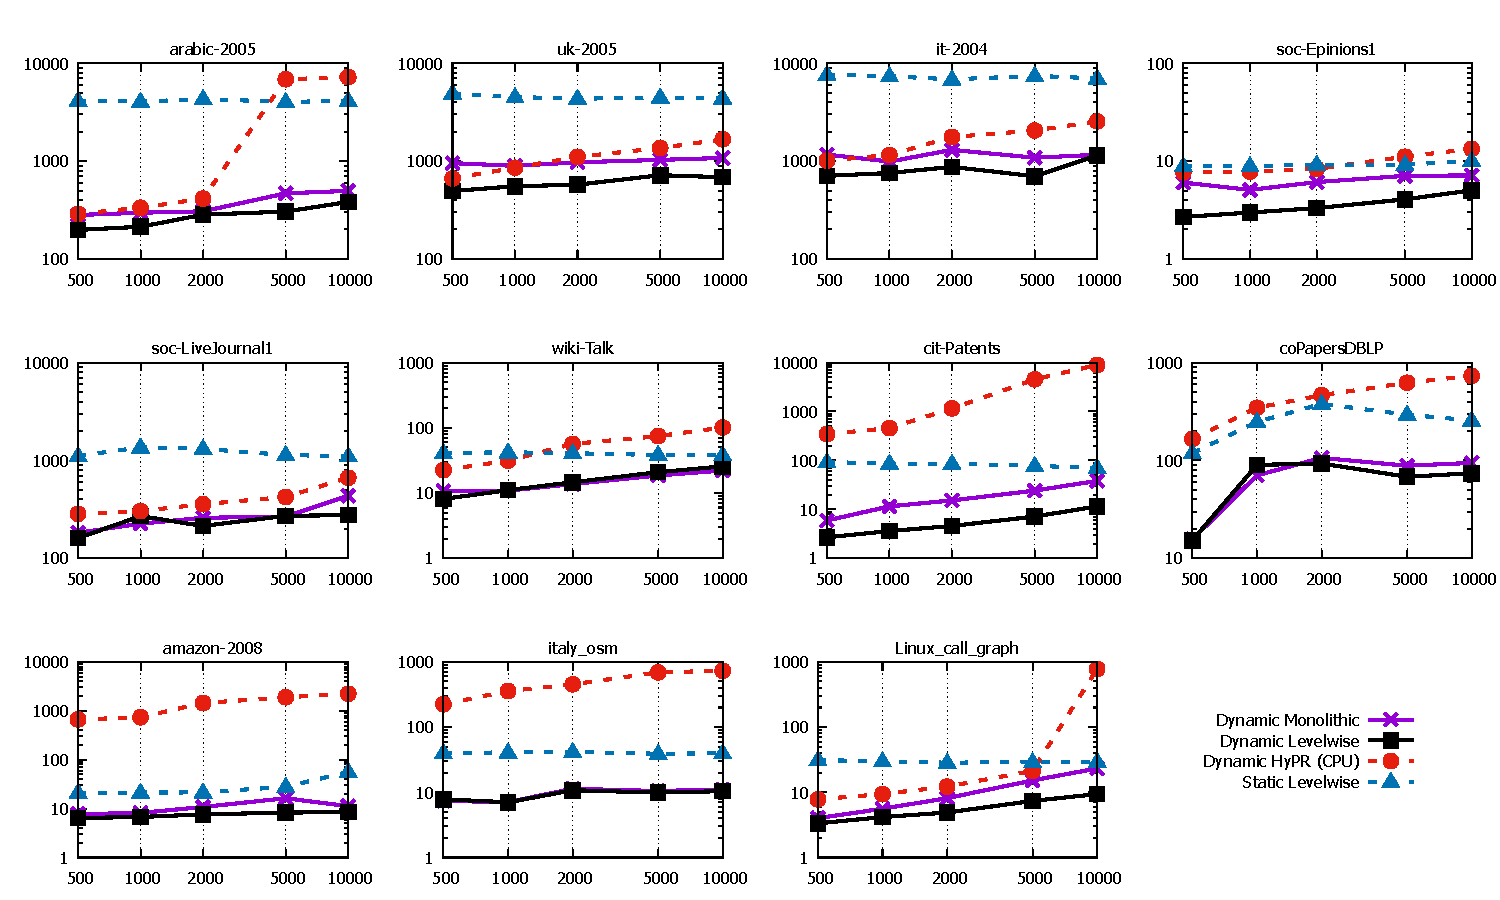
\includegraphics[width=1.00\textwidth]{out/time-omp-all.pdf}};
    \draw (-9.1, 0) node {\rotatebox[origin=t]{90}{Runtime (ms)}};
    \draw (0, -5.7) node {\rotatebox[origin=t]{0}{Batch size}};
  \end{tikzpicture}
  \caption{Time taken for PageRank computation using \monolithicPR{} and \levelwisePR{} on the CPU. Batch sizes of 500, 1000, 2000, 5000, and 10000 are used. Time taken with \emph{pure CPU implementation of HyPR} and \emph{plain STIC-D PageRank (static Levelwise)} is also included for comparison.}
  \label{fig:time-omp-all}
\end{figure*}
